\documentclass[a4paper,10pt]{article}
\usepackage[utf8]{inputenc}
\usepackage{enumitem}
\usepackage[top=40mm, bottom=40mm, left=20mm, right=20mm]{geometry}
\usepackage{graphicx}
\usepackage[absolute]{textpos}
\usepackage{wrapfig}
\usepackage{hyperref}

\title{\vspace{-4cm}Curriculum Vitae}
\date{}

\begin{document}

\maketitle

\begin{textblock}{6}(9, 1.5)
    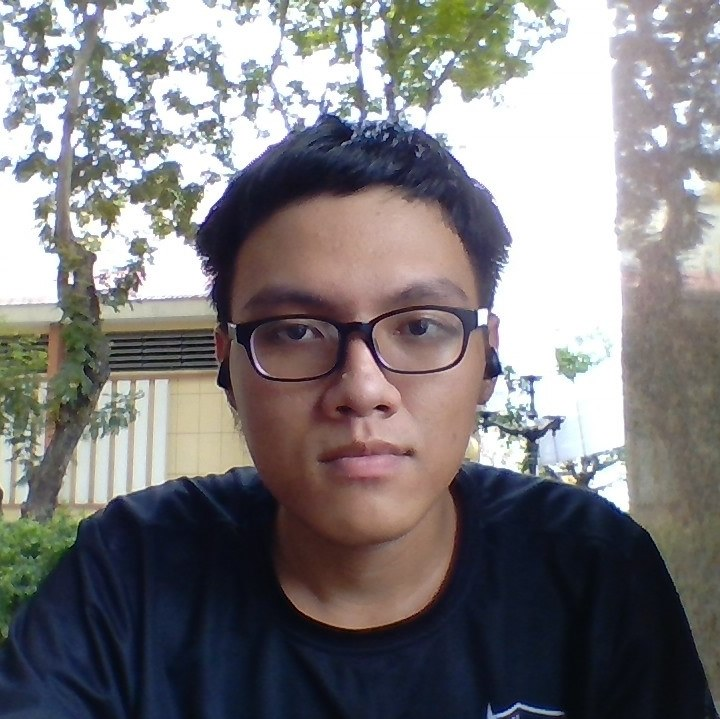
\includegraphics[width=0.8\textwidth]{a.jpg}
\end{textblock}

\section*{Personal Information}

\begin{itemize}
    \item Name: Dat Le-Duc
    \item Position: Python AI/ML/NLP Engineer Intern
    \item Phone: (+84) 888.514.045
    \item Email: dat20026969@gmail.com
    \item Facebook: \href{https://www.facebook.com/Datridosati}{Datridosati}
    \item LinkedIn: \href{https://www.linkedin.com/in/dat-le-duc-96824112b}{dat-le-duc-96824112b}
    \item GitHub: \href{https://github.com/dat20026969}{dat20026969}
\end{itemize}

\section*{Career Objective}

I am a third-year student at my university, seeking to gain hands-on experience in an innovative and challenging IT environment where I can utilize my skills in Python, AI, Machine Learning, and Natural Language Processing.

\section*{Skills}

\begin{itemize}
    \item Proficient in Python, C++, Mathematics.
    \item Strong understanding of machine learning and natural language processing concepts
    \item Experience working with AI/ML/NLP libraries such as TensorFlow, PyTorch, NLTK, etc.
    \item Quite good knowledge of software development methodologies, tools, and processes
    \item Proficient in tools like Git, GitHub, Google Colab, Jupyter Notebook
    \item Language Skills: English (IELTS 5.5), Vietnamese (Native)
\end{itemize}

\section*{Education}

\textbf{Bachelor of Science in Information Technology}, Ho Chi Minh University of Science (2020-present)
\\
\textbf{GPA: } 2.7/4
\\
\textbf{Luong Van Chanh high school for the gifted}, Mathematics Specialized Class (2017-2020)

\section*{Projects}

\begin{itemize}
    \item \textbf{Project 1:} Computer Vision mini-projects: Face-Object Recognition by Camera, Image-2-text, Images Similarity
    \item \textbf{Project 2:} Research Text Classification with BERT in NLP
    \item \textbf{Project 3:} Research review scientific articles about chatGPT: ChatGPT: Beginning of an End of Manual Linguistic Data Annotation? Use Case of Automatic Genre Identification
\end{itemize}

\section*{Courses and Certificates}

\begin{itemize}
    \item \textbf{Course/Certificate 1:} Big-O GREEN - Big-O Coding Center (1/2021-3/2021)
    \item \textbf{Course/Certificate 2:} Big-O BLUE - Big-O Coding Center (5/2021-7/2021)
    \item \textbf{Course/Certificate 3:} Big-O ORANGE - Big-O Coding Center (10/2021-12/2021)
    \item \textbf{Course/Certificate 4:} Foundation of Machine Learning - VietAI
    (10/2020 - 5/2023)
    \item \textbf{Course/Certificate 5:} ALL-IN-ONE from AI VIETNAM (5/2023 - now)
    
\end{itemize}

\section*{Awards and Achievements}

\begin{itemize}
    \item \textbf{Consolation Prize,} Iran Geometry Olympiad (IGO), 2017, 2018
    \item \textbf{Consolation Prize,} American Mathematics Competition, 2017, 2018
    \item \textbf{Miscellaneous,} Participated and won several prizes in Mathematics and English competitions, both online and paper-based, in the past.
\end{itemize}

\section*{Activities}

\begin{itemize}
    \item \textbf{Activity 1:} MTI Online Hackathon Game Jam (2020)
    \item \textbf{Activity 2:} SEA Culture Competition in Ho Chi Minh Open University (10/2022-11/2022)
\end{itemize}

\section*{Additional Information}

\begin{itemize}
    \item \textbf{Hobbies:} Sports and Games
    \item \textbf{Personalization:} Reserved, kind, enthusiastic and passionate about work and dreams
\end{itemize}

\end{document}
